\documentclass{bmvc2k}

%% Enter your paper number here for the review copy
\bmvcreviewcopy{536}

\usepackage{amsfonts,amssymb} 
\usepackage{subfigure}
\usepackage{booktabs}
\usepackage{diagbox}
\usepackage{graphicx}
\usepackage{multirow}
\usepackage{amsmath}
\usepackage{overpic}
\usepackage[linesnumbered,ruled,vlined]{algorithm2e}


\title{3D Object Detection and Tracking on Streaming Data}

% Enter the paper's authors in order
% \addauthor{Name}{email/homepage}{INSTITUTION_CODE}
\addauthor{Xusen Guo}{guoxs3@mail2.sysu.edu.cn}{1}
\addauthor{Jianfeng, Gu}{gujf5@mail2.sysu.edu.cn}{1}
\addauthor{Chengzhang, Yang}{yangchzh5@mail2.sysu.edu.cn}{1}
\addauthor{Zixiao Xu}{xuzx5@mail2.sysu.edu.cn}{1}
\addauthor{Silu Guo}{guoslu@mail2.sysu.edu.cn}{1}
\addauthor{Shuoxuan Han}{hanshx@mail2.sysu.edu.cn}{1}
\addauthor{Kai Huang}{huangk36@mail.sysu.edu.cn}{1}

% Enter the institutions
% \addinstitution{Name\\Address}
\addinstitution{
	Key Laboratory of Machine Intelligence\\
	and Advanced Computing, Ministry of \\
	Education School of Data and Computer Science, Sun Yat-Sen \\
	University, GuangZhou, China
}

\runninghead{XuSen Guo, KaiHuang, SYSU}{3D Object Detection and Tracking on Streaming Data}

% Any macro definitions you would like to include
% These are not defined in the style file, because they don't begin
% with \bmva, so they might conflict with the user's own macros.
% The \bmvaOneDot macro adds a full stop unless there is one in the
% text already.
\def\eg{\emph{e.g}\bmvaOneDot}
\def\Eg{\emph{E.g}\bmvaOneDot}
\def\etal{\emph{et al}\bmvaOneDot}

%-------------------------------------------------------------------------
% Document starts here
\begin{document}
\maketitle
\begin{abstract}
Recent approaches for 3D object detection have made tremendous progress due to the development of neural networks. However, previous researches are mostly single frame based, information between frames is scarcely explored. In this paper, we attempt to leverage the temporal information in streaming data and explore 3D object detection as well as tracking based on multiple frames. Towards this goal, we set up a ConvNet architecture that can associate multi-frame images and multi-frame point clouds to generate accurate 3D detections and trajectories in an end-to-end form. Specifically, a correlation module is introduced to capture objects co-occurrences across time, and a multi-task objective for frame-based object detection and across-frame track regression are used. Our proposed architecture is proven to produce competitive results on the KITTI Object Tracking Benchmark, with 72.21\% in MOTA and 82.29\% in MOTP respectively.
\end{abstract}

%-------------------------------------------------------------------------
\section{Introduction}
\label{sec:intro} 
3D Object detection has received increasing attention over the last few years due to the rapid development of autonomous driving. Compared to 2D image, 3D information can provide accurate localization of targets and characterize their shapes. Current approaches for 3D object detection are mostly carried out in three fronts: image based\cite{7780605, chen20183d}, point clouds based\cite{zhou2018voxelnet,yang2018pixor,simon2018complex}, and multi-view fusion based\cite{chen2017multi,ku2018joint}. Most of these approaches have achieved competitive results but are limited to single frame input.

%2. In autonomous driving, the data we can obtain naturally is always streaming. Thus performing object detection in streaming data is more straightforward for most applications. Compared to single frame input, the temporal features in streaming data provide the consistency between neighboring frames, which can reduce the noise over time. Moreover, truncated and occluded targets can benefit more from streaming data. Therefore, exploring 3D object detection methods specifically for streaming data is essential and promising.

During autonomous driving, data are always generated in a streaming fashion and thus it is more natural to perform object detection from streaming data. Compared to single-frame based approaches, streaming data can provide consistent temporal correlations between consecutive frames for detected features, which can reduce detection noise over time. In addition, truncated and occluded targets can possibly be compensated by subsequent frames within streaming data. Therefore, exploring 3D object detection methods specifically for streaming data is essential and promising.

%1. In autonomous driving, streaming data is more natural and straightforward than single frame data. Fast and accurate 3D object detection in streaming data is crucial for most autonomous driving scenarios. However, applying existing single frame based approaches directly to streaming data will inevitably loss the consistency between frames, and also introduces unaffordable computational costs for most applications. Therefore, exploring 3D object detection methods specifically for streaming data is essential and promising.

% Performing 3D object detection in streaming data is however complicated. The first difficulty is that the hardness in acquiring 3D information. Camera data provides richness appearance features but lack of depth information. While LiDAR can accurately detect the position of object of interest, it is difficult to determine the appearance of object purely from its point cloud representation. Moreover, the sheer numbers of frames that streaming data provides introduces unaffordable computational costs for frame level detection. Additionally, due to the difficult in determining the corresponding points between frames, 3D scene flow estimation for temporal feature representation is challenging. 

Performing 3D object detection in streaming data is however complex. First of all, acquiring consistent 3D information between frames is difficult. On the one hand, camera data provide rich appearance features but lack of depth information. On the other hand, though LiDAR can accurately detect the position of object of interest, it is difficult to determine the appearance of object purely from its point cloud representation. Second, how to correlate the features between individual frames is not obvious. For example, generating 3D scene flow with temporal feature representation will need to determine the corresponding points between frames, which is not straightforward and challenging. Last but not least, the sheer numbers of frames that streaming data provide introduces unaffordable computational costs for frame level detection. 

%Like extend 2D object detection to 3D scenes, one can also extend video object detection to 3D streaming data. However, using camera data only and performing video-based approaches for 3D streaming object detection is challenge, since those methods unable utilize depth information and suffer from motion blur and partial occlusion. While devices such as LiDAR which generate point clouds can mitigate these issues by accurately detecting the position of object of interest, it is difficult to determine the appearance of object purely from their point cloud representation. Additionally,  due to the difficult in determining the corresponding points between frames, accurate 3D scene flow estimation involved in temporal feature representation is challenge.  

In this paper, we propose a dual-way network named Bi-AVOD to tackle the aforementioned problem. Our network is based on an aggregate view object detection architecture AVOD \cite{ku2018joint} and the structure is illustrated in \figurename \, \ref{fig:bi-avod}. The network takes two adjacent frames (i.e. an image combined with its corresponding point cloud) as inputs and is capable of fusing different features in image and point cloud, thus utilizing the strengths of both. In order to avoid estimating 3D scene flow directly, a correlation module is aided to our Bi-AVOD for temporal feature encoding. The correlation module computes convolutional cross-correlation between the features response of adjacent frames to estimate local displacements. Moreover, for a fast inference speed, we perform 3D object detection on key frames and propagate predicted bounding boxes to neighboring frames for a streaming-based detection. Furthermore, by linking detections over time with local displacement information, multi-object tracking can be performed through \textit{tracking by detection} \cite{lenz2015followme}. 

%With detections of key frames and corresponding local displacements, 3D streaming object detection can be implemented by propagating detections to neighboring frames.  Furthermore, by linking detections over time with local displacement information, multi-object tracking can be performed through \textit{tracking by detection} \cite{lenz2015followme}. 

In summary, our contributions are threefold: 
\textit{(i)} we set up a dual-way network for 3D streaming-based object detection and multi-object tracking in autonomous driving scenarios. \textit{(ii)} Instead of encoding temporal feature using 3D scene flow, we introduce a correlation module to compute convolutional cross-correlation of adjacent frames for temporal feature representation. \textit{(iii)} We perform our approach to KITTI Object Tracking Benchmark and obtain competitive results, with 72.21\% in MOTA and 82.29\% in MOTP respectively.

%Inspired by \cite{feichtenhofer2017detect}, we transform AVOD \cite{ku2018joint} structure into a dual-way network with an embedded correlation module, named Bi-AVOD. The network takes two adjacent key frames (i.e. an image combined with its corresponding point cloud) as inputs and predicts locations and orientations of objects as well as their local displacements between frames. Note that Bi-AVOD is an aggregate view object detection architecture capable of fusing different features in image and point cloud, thus utilizing the strengths of each. 

% The aforementioned problems can be mitigated by combining the information obtained by camera and LiDAR.

% Though approaches such as \cite{liu2018learning, behl2018pointflownet} have been presented to learn 3D motion field in the world, their performance is limited when it comes to large and complex scenes.
%
%Most modern video object detection approaches require optical flow information, for example, \cite{zhu2017flow,zhu2018towards} associate vision feature and optical flow to build an accurate end-to-end learning framework for video object detection.

%While another choice is to use LiDAR data, since point clouds provide an accurate spatial representation of the world allowing for precise positioning of objects of interest, thus the problem of motion blur and occlusion would be avoided in three-dimensional perspective. Nonetheless, LiDAR does not capture appearance well when compared to the richness of images, moreover, accurate 3D scene flow estimation from point clouds is tremendously tough. Though approaches such as \cite{liu2018learning, behl2018pointflownet} have been presented to learn 3D motion field in the world, their performance is limited when it comes to large and complex scenes. 
%-------------------------------------------------------------------------
%\vspace{-0.2cm}
\section{Related Work}
\label{sec:related work}

\textbf{3D object detection.} Currently, most approaches in 3D object detection can be divided into three types: image based detectors, point cloud based detectors, and fusion based detectors. Images based approaches such as Mono3D \cite{7780605} and 3DOP \cite{chen20183d} use camera data only. Since image lacks depth information, hand-crafted geometric features are required in these approaches. Point cloud based methods are usually done in two fronts: voxelization based and projection based, according to how point clouds information is represented. Voxelization based methods utilize a voxel grid representation to encoder the point cloud and then apply a 3D CNN for feature extraction. These approaches include 3D FCN \cite{li20173d}, Vote3Deep \cite{engelcke2017vote3deep}, VoxelNet \cite{zhou2018voxelnet}, \etal These approaches suffer from the sparsity of point cloud and enormous computation costs in 3D convolution. While projection based methods attempt to project point cloud to a perspective view (e.g. bird eye view) and apply image-based feature extraction techniques, such as PIXOR \cite{yang2018pixor}, FaF \cite{luo2018fast}, Comple-YOLO \cite{simon2018complex}, \etal These methods take advantage of the fact that 3D detections in driving scenes are almost on the same plane, thus loss of height information has little influence on performance. However, due to the sparsity of point cloud, features after projection are insufficient for accurate object detection, especially for small targets. 

Fusion based approaches such as F-PointNet \cite{qi2018frustum} first extracts the 3D bounding frustum of an object by extruding 2D bounding boxes from image detectors, then consecutively performs 3D object instance segmentation and amodal extent regression to estimate the amodal 3D bounding box. This method works well for indoor scenes and brightly lit outdoor scenes, but are expected to perform poorly in more extreme outdoor scenarios. MV3D \cite{chen2017multi} extends the image based RPN of Faster R-CNN\cite{ren2015faster} to 3D and proposes a 3D RPN, then applies feature fusion of images and point clouds to produces accurate 3D detections. However, due to the insufficient information in feature extraction caused by downsampling, it does not work well for small targets. AVOD \cite{ku2018joint} is similar to MV3D in 3D RPN and feature fusion, but with  full resolution feature maps produced by a pyramid architecture, which leads to a great improvement in localization accuracy for small targets. In our proposed approach, the AVOD framework is used as a basic 3D object detection module.

\textbf{Video object detection.} Nearly all existing methods in video object detection incorporate temporal information on either feature level or final box level. FGFA \cite{zhu2017flow} leverages temporal coherence on feature level. The network first applies feature extraction network on individual frames to produce per-frame feature maps, and then enhances features at a reference frame by warping the nearby frames feature maps according to flow emotion. On the other hand, final box level approaches usually utilize temporal information in bounding box post processing. T-CNN \cite{kang2018t, kang2016object} leverages precomputed optical flows to propagate predicted bounding boxes to neighboring frames, and then generates tubelets by applying tracking algorithms from high-confidence bounding boxes. Seq-NMS \cite{han2016seq} improves NMS algorithm for video by constructing sequences along nearby high-confidence bounding boxes from consecutive frames. While boxes of the sequence are then re-scored to the average confidence and other boxes close to this sequence are suppressed. 

Other approaches attempt to learn temporal information between consecutive frames to avoid using optical flow. D\&T \cite{feichtenhofer2017detect} presents an end-to-end fully convolutional architecture, it uses a detection and tracking based loss for simultaneous detection and tracking in video. In order to learn temporal information representation, the network is fed with multiple frames, and a correlation module is embedded for computing convolutional cross-correlation between frames. Our Bi-AVOD approach is mainly inspired by D\&T. 

\textbf{3D multi-object tracking.} Existing 3D multi-object tracking methods are mostly implemented based on tracking by detection. For example, FaF \cite{luo2018fast} jointly reasons about 3D detection, tracking and motion forecasting taking a 4D tensor created from multiple consecutive temporal frames. It can aggregate the detection information for the past $n$ timestamps to produce accurate tracklets. DSM \cite{frossard2018end} first predicts 3D bounding boxes in continuous frames and then associates detections using a \textit{Matching net} and a \textit{Scoring net}, which is similar to our approach. However, their 3D detector is directly single frame based approach MV3D\cite{chen2017multi}, temporal features between frames are mostly ignored. Moreover, their bounding boxes association is done by solving a linear program, while ours by applying a improved IOU tracker algorithm based on \cite{bochinski2018extending}. 

%FGFA \cite{zhu2017flow} leverages temporal coherence on feature level, it first applies feature extraction network on individual frames to produce the per-frame feature maps, and then enhance the features at a reference frame by warping the nearby frames feature maps according to the flow emotion, finally, the detection network performs object detection only on the reference frames. Later a more efficient approach based on FGFA has been presented in \cite{zhu2018towards}, it introduces three new techniques, sparsely recursive feature aggregation, spatially-adaptive partial feature updating and temporally-adaptive key frame scheduling, which make this unified approach faster, more accurate and more flexible.

%-------------------------------------------------------------------------
\begin{figure*}
	\rule{0pt}{1ex}
	\setlength{\abovecaptionskip}{-1.5cm}
	\begin{center}
		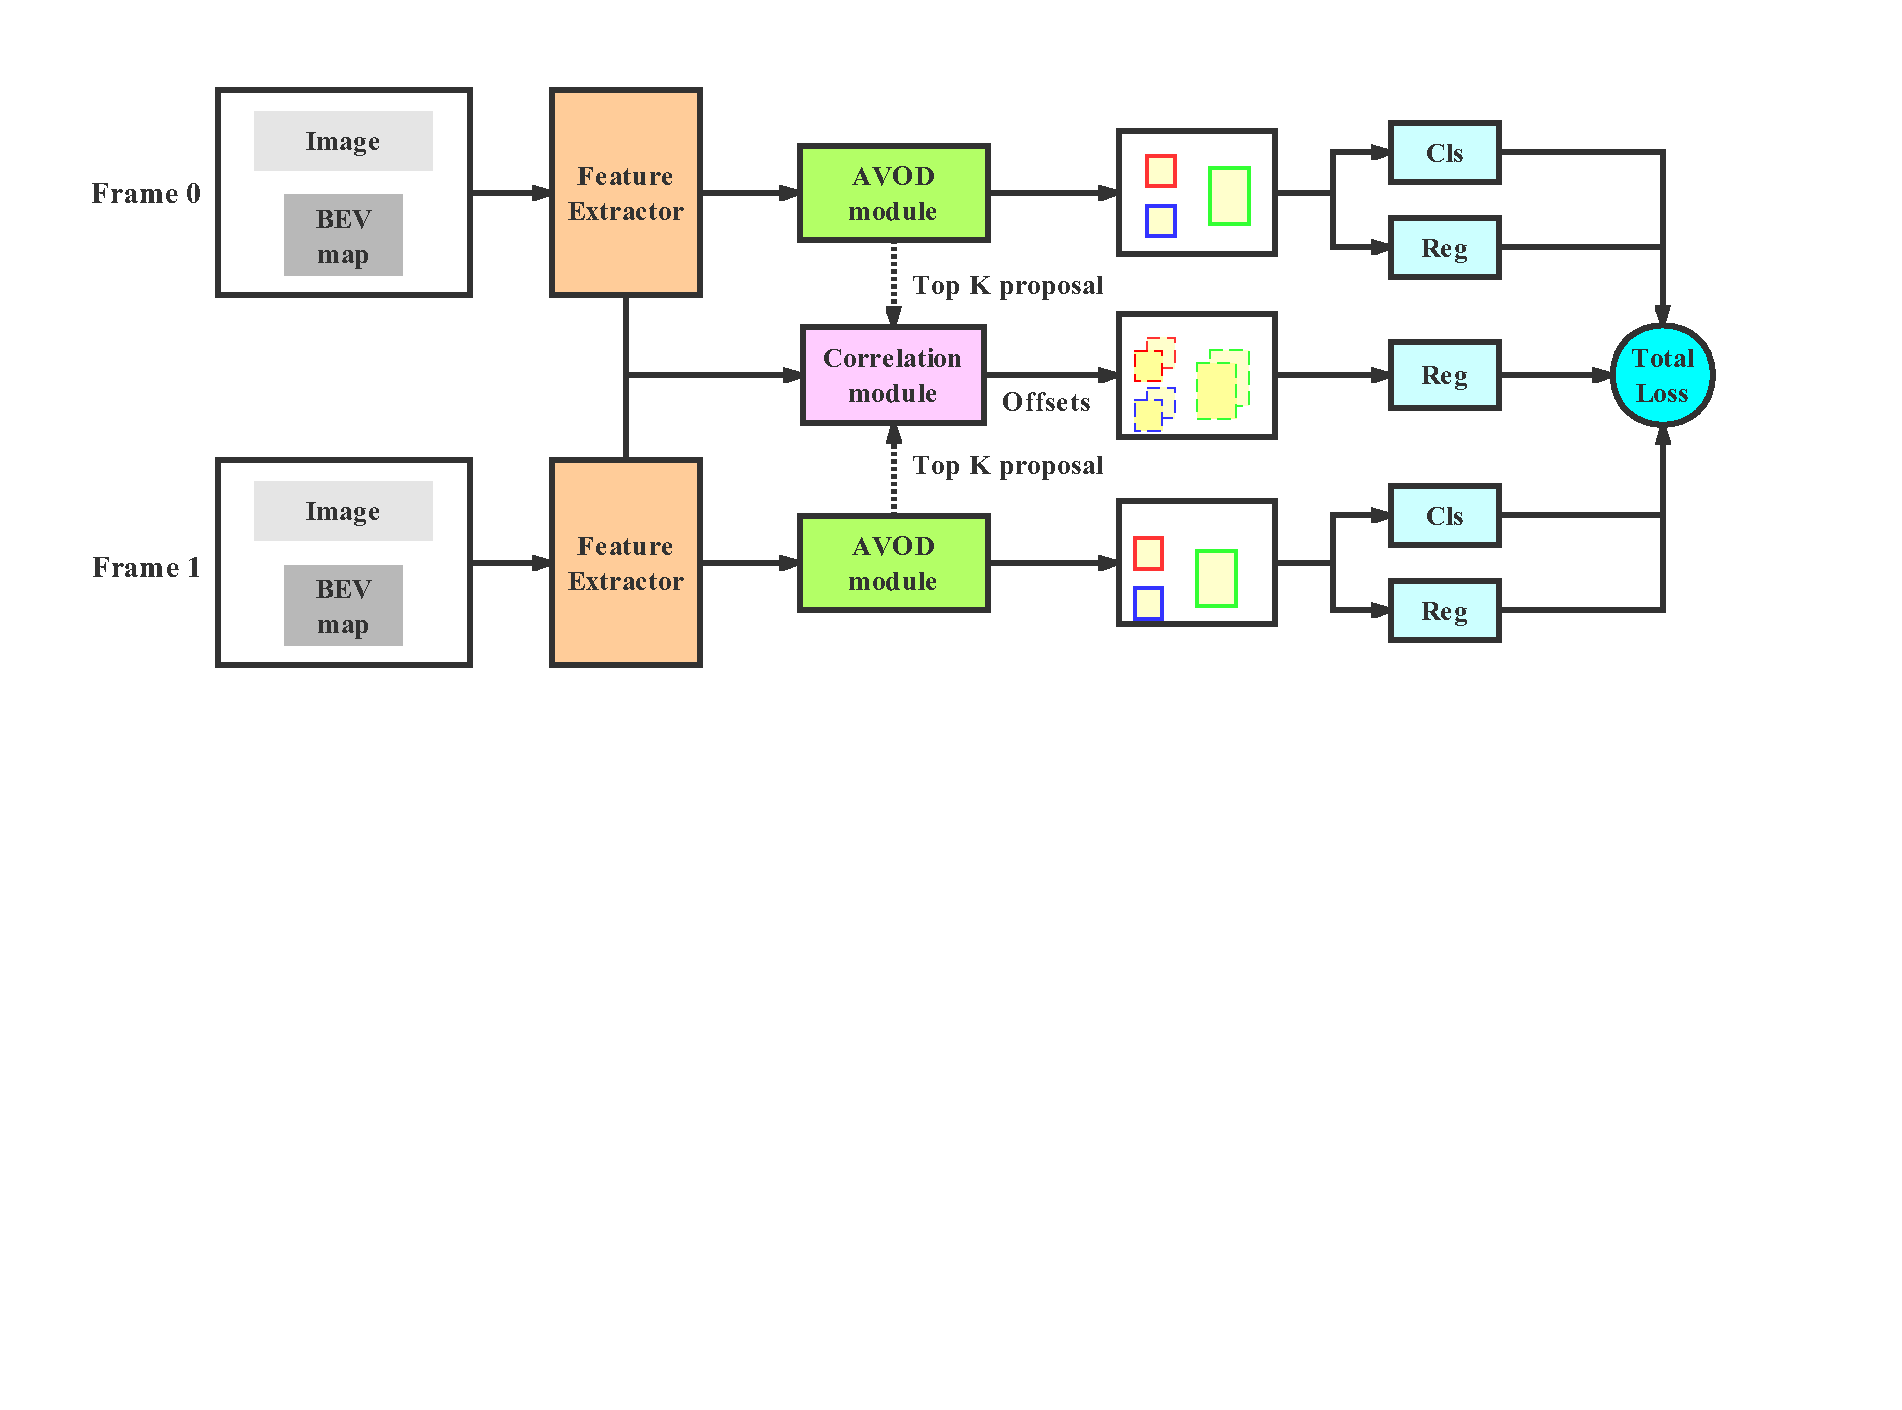
\includegraphics[trim={0cm, 10cm, 3cm, 1cm}, clip, width=\textwidth]{images/Bi-AVOD.pdf}
	\end{center}
	\caption{Bi-AVOD architecture. For convenience, AVOD module here does not include feature extractor and loss function.}
	\label{fig:bi-avod}
	\vspace{-0.5cm}
\end{figure*}

\begin{figure*}
	\setlength{\abovecaptionskip}{-0.5cm}
	\begin{minipage}[t]{0.5\linewidth}
		\centering
		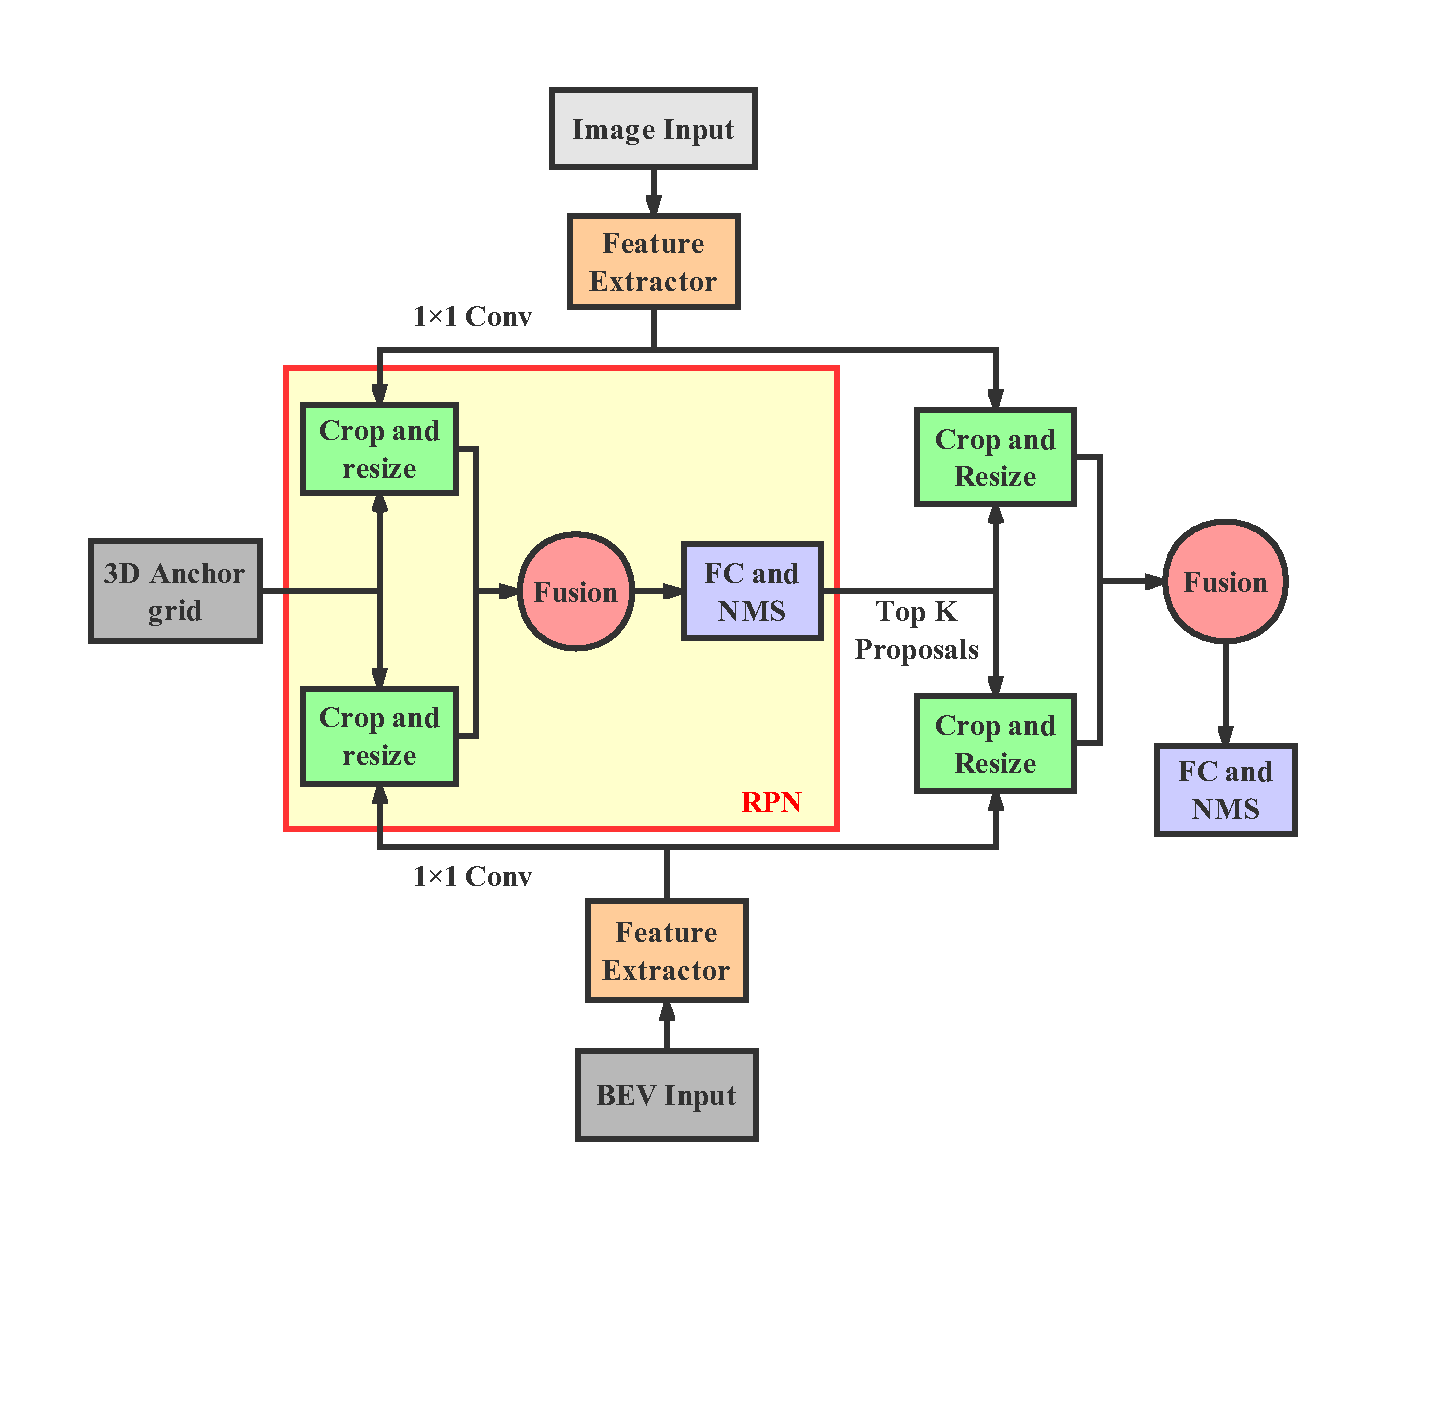
\includegraphics[trim={0cm, 4cm, 2cm, 0cm}, clip, width=2.7in]{images/AVOD.pdf}
		\caption{AVOD architecture}
		\label{fig:avod}
	\end{minipage}%
	\begin{minipage}[t]{0.5\linewidth}
		\centering
		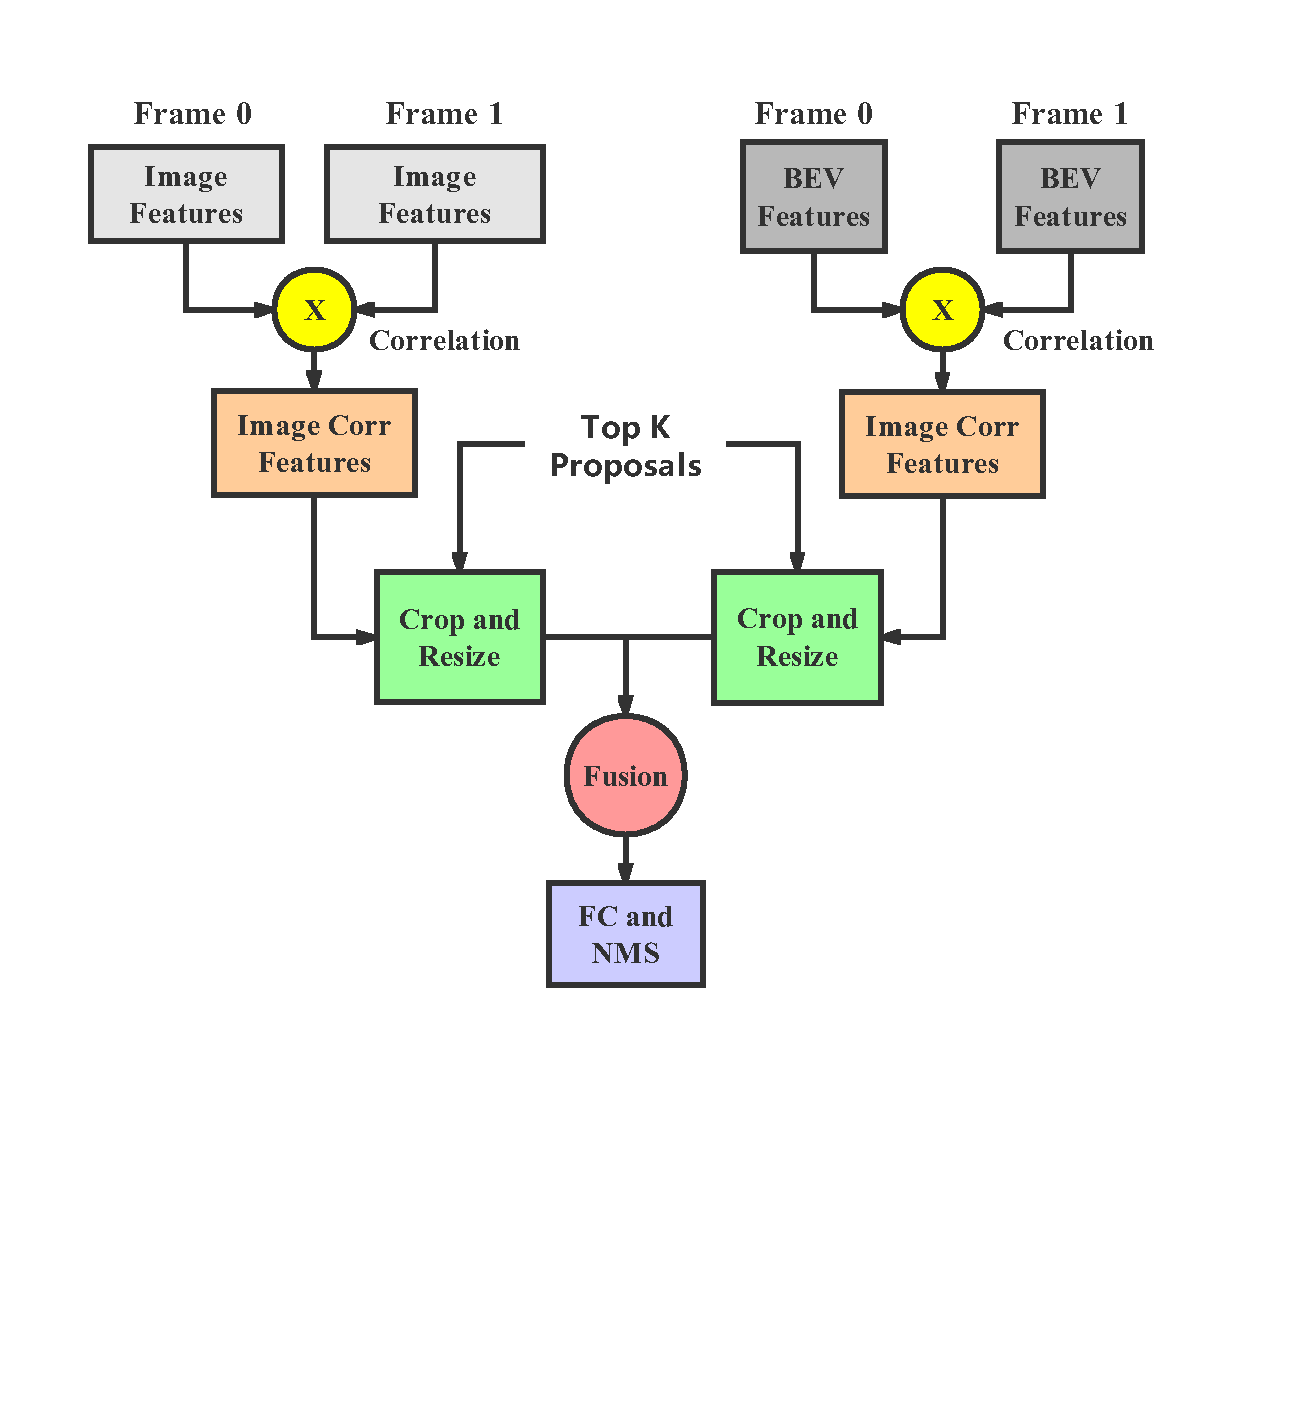
\includegraphics[trim={0cm, 6cm, 2cm, 0cm}, clip, width=2.6in]{images/Correlation.pdf}
		\caption{Correlation module}
		\label{fig:correlation}
	\end{minipage}
\end{figure*}

\section{Methodology}
\label{sec:method}
In this section we first give an overview of our Bi-AVOD approach (Sec. 3.1) that generates object detection results and tracklets given two adjacent key frames as inputs. We then introduce the correlation module (Sec. 3.2) that predicts the displacement of corresponding targets in two adjacent key frames. Sec. 3.3 shows the multi-task objective function. Sec. 3.4 shows how we implement 3D streaming object detection and multi-object tracking with network outputs.

\subsection{Bi-AVOD model structure}
We aim at performing 3D object detection and tracking on streaming data. To this end, we transform AVOD\cite{ku2018joint} architecture to a dual-way network. \figurename \, \ref{fig:bi-avod} illustrates our Bi-AVOD architecture. By doubling its input, we can feed two adjacent key frames (image and point cloud) simultaneously and obtain corresponding object detection results. Meanwhile, the local displacements can be estimated by computing convolutional cross-correlation between the features responses of adjacent frames using correlation module. With predicted detections of two key frames and their local displacements, interpolation algorithms can be performed to propagate detections to neighboring frames. Also, 3D multi-object tracking can be implemented by applying box association algorithm. Note that two \textit{Feature Extractors} and two \textit{AVOD modules} in \figurename \, \ref{fig:bi-avod} are parameter sharing, thus the increased computational costs only come from the correlation module. We will simply review the AVOD architecture in this section, and the correlation module will be left to next section.

AVOD\cite{ku2018joint} architecture is proposed for 3D object detection in autonomous driving by aggregating front view image and BEV feature maps generated by LiDAR data. It is a two-stage method, the architecture is illustrated in \figurename \, \ref{fig:avod}. First, pyramid based feature extractors are used to generate full resolution feature maps of both BEV map and RGB image inputs; both feature maps are then fed to a fusion RPN to generate \textit{Top K} non-oriented region proposals after applied a $1 \times 1$ convolution for dimensionality reduction. Note that the default anchors in images and BEV feature maps are generated through 3D anchor grid projection, and ROI Pooling is implemented by \textit{Crop and Resize} operations. Finally, the \textit{Top K} proposals are passed to the detection network for dimension refinement, orientation estimation and category classification. We refer the reader to \cite{ku2018joint} for further understanding of the architecture.

\subsection{Correlation module}
Our 3D correlation module is illustrated in \figurename \, \ref{fig:correlation}. Given feature maps of two adjacent key frames, it first performs correlation operation to compute convolutional cross-correlation. Similar to RPN sub-module in AVOD, the module then extracts feature crops via multiview \textit{Crop and Resize} operations guided by aforementioned \textit{Top K} non-oriented region proposals. The feature crops are then fed to a fusion module to generate multiview aggregated features. The fusion module is identical to the one involved in AVOD, which was first introduced in MV3D\cite{chen2017multi}. The aggregated features are then passed to a fully connected layer for regression. After that, non-maximum suppression (NMS) is applied to ignore redundant, overlapping bounding boxes for the final loss calculation.

Similar to FlowNet \cite{dosovitskiy2015flownet}, we restrict correlation operation to a local neighborhood instead of all possible circular shifts in a feature map. This restriction helps the module avoid large output dimensionality. The correlation operation performs point-wise feature comparison of two feature maps $f_t$, $f_{t+\tau}$ by
\begin{equation}
\mathcal{C}^{t, t+\tau}(i, j, p, q) = \Big \langle f_t(i, j), f_{t+\tau} (i+p, j+q) \Big \rangle \label{con:correlation}
\end{equation}
where $p, q \in [-d, d]$ are offsets to compared features in a local square window defined by the maximum displacement $d$, and $i, j$ are the location of the window center in a feature map. The output is a correlation feature map of size $\mathcal{C} \in \mathbb{R}^{h \times w \times (2d+1) \times (2d+1)}$, where $h, w$ are the height and the width of the feature map.

After applying \eqref{con:correlation}, two correlation feature maps are obtained, one for point cloud $\mathcal{C}^{t, t+\tau}_{pc}$, and one for RGB image $\mathcal{C}^{t, t+\tau}_{img}$. ROI pooling and feature fusion are then performed to produce aggregate feature map $\mathcal{C}^{t,t+\tau}_{fusion} = fusion(\mathcal{C}^{t, t+\tau}_{pc}, \mathcal{C}^{t, t+\tau}_{img})$, which is then flattened and fed to a fully connected layer to predict the transformation $\Delta^{t, t+\tau} = (\Delta^{t,t+\tau}_{x}, \Delta^{t,t+\tau}_{y}, \Delta^{t,t+\tau}_{z}, \Delta^{t,t+\tau}_{r})$ of the RoIs from $t$ to $t+\tau$. We hold the prior that the size of a target does not change over time, thus the network only needs to predict the variations in the center coordinates and steering angle.

\subsection{Multitask detection and correlation objective}
We extend the multi-task loss of object detection, consisting of a classification loss $L_{cls}$ and a regression loss $L_{reg}$, with an additional term $L_{corr}$ that scores the displacement regression between corresponding objects across two frames. Considering a batch of $N$ RoIs after category balanced sampling, the network predicts softmax probabilities $\{p_i\}^N_{i=1}$, bounding box regression offsets $\{b_i\}^N_{i=1}$, and cross-frame displacement regression $\{\Delta^{t+\tau}_i\}^{N_{corr}}_{i=1}$, the overall objective function is shown as:
\begin{equation}
\begin{split}
L(\{p_i\}, \{b_i\}, \{\Delta_i\}) = \frac{1}{N} \sum^N_{i=1} L_{cls}(p_{i, c^*}) 
+ \frac{\alpha}{N_{fg}}\sum^N_{i=1} [c^*_i > 0]L_{reg}(b_i, b^*_i) \\
+ \frac{\beta}{N_{corr}} \sum^{N_{corr}}_{i=1}L_{corr}(\Delta^{t+\tau}_i, \Delta^{*, t+\tau}_i)
\end{split}
\end{equation}
where $c^*_i$ is the ground truth class label of an RoI and $p_{i, c^*_i}$ is corresponding predicted softmax score. $b^*_i$ is the ground truth of bounding box regression target, and $\Delta^{*, t+\tau}_i$ is the ground truth of displacement regression target. The indicator function $ [c^*_i > 0]$ is 1 for foreground RoIs and 0 for background RoIs. $L_{cls}$ is cross-entropy loss, and $L_{reg}$, $L_{corr}$ are smooth L1 loss \cite{girshick2015fast}. $\alpha$ and $\beta$ are weight coefficients for $L_{reg}$ and $L_{corr}$, in this work we set 5 and 1 respectively. Note that we only consider the $N_{fg}$ foreground RoIs loss for $L_{reg}$, and $L_{corr}$ is active only for foreground RoIs which have a track correspondence in both frames. Additionally, $b^*_i$ and $ \Delta^{*, t+\tau}_i$ are all encoded following \cite{ku2018joint}.

\subsection{3D streaming object detection and tracking}
Given a sequence of $N$ frames $\{I_f \mid f = 1, ..., N\}$, streaming-based object detection task needs to predict a set of detections $D_f$ for each frame $I_f$, where $D_f = \{d^i_f \mid i = 1,...N_f\}$, $d^i_f$ is $i^{th}$ target and $N_f$ is the number of targets in frame $f$. Note that $D_f$ can also be an empty set when no target is detected in a frame. In 3D object detection, each detection $d_i$ is parametrized as $D_i = (x_i, y_i, z_i, w_i, h_i, l_i, \theta_i, s_i)$, where $(x_i, y_i, z_i)$ corresponds to the coordinate of target center, $(w_i, h_i, l_i)$ corresponds to width, height, length of the target, $\theta_i$ the rotation angle in yaw axis and $s_i$ prediction confidence of the target.

We only perform object detection in key frames due to the redundant features in streaming data. Detections of the intermediate frame can be determined leveraging the detection results of its adjacent key frames. Suppose we have two predicted detections set $(D_f, D_{f+\tau})$ of two consecutive key frames $(I_f, I_{f+\tau})$, where $\tau$ is temporal stride, the detection result $d^i_{f+t}$  of intermediate frame $I_{f+t} (t \in \{1, \tau-1\})$ can be obtained by
\begin{equation}
d^i_{f+t} = \mathcal{F}(W_f d^i_f, W_{f+\tau} d^i_{f+\tau}) \label{con:interpolation}
\end{equation}
where $W_f, W_{f+\tau}$ are the corresponding weight coefficients and $\mathcal{F}$ is interpolation function. Note that we can use Equation \eqref{con:interpolation} to generate $d^i_{f+t}$ only when the target exists in $D_f$ and $D_{f+\tau}$ simultaneously. If a target is the start or end of a trajectory in intermediate frames, this method will fail. Although carefully selecting key frames could fix this problem, it is beyond the scope of this work. In this paper we focus on the targets that always exist between two key frames.

For multi-object tracking, we attempt to assign each detection in each frame to a unique trajectory $T_k = \{d^k_{f_1}, d^k_{f_2}, ..., d^k_{f_{N_k}}\}$, utilizing an improved IOU tracker algorithm\cite{bochinski2018extending} (detailed description is available in supplementary material). Where $k$ is the trajectory id and $N_k$ is the length of $T_k$. Unlike multi-object tracking in 2D image which suffers from boxes overlap, detection in 3D has its unique position, any overlap of two detections in 3D means high probability of the same target. Thus a IOU based data association algorithm can also work well in our approach.
%-------------------------------------------------------------------------

\section{Experiments}
\label{sec:experiments}

\subsection{Datasets and Training}

\textbf{Datasets.} We use KITTI object tracking Benchmark \cite{geiger2013vision} for evaluation. It consists of 21 training sequences and 29 test sequences with vehicles annotated in 3D. Each sequence includes hundreds of point cloud frames captured by Velodyne HDL-64E rotating 3D laser scanner and corresponding RGB images. We split 21 training sequences into two parts according to their sequence number, odd numbered sequences for training datasets and even numbered ones for evaluation datasets. For multi-object tracking evaluation, we train our model in all 21 training sequences.

\textbf{Datasets preprocessing.} Similar to the data preprocessing in \cite{ku2018joint}, we crop point clouds at $[-40, 40] \times [0, 70] \times [0, 2.5]$ meters along $Y, X, Z$ axis respectively to contain points within the field of view of the camera. In KITTI tracking datasets, the observer is an autonomous vehicle, thus the coordinate system of consecutive frames shift due to the movement of the observer over time. Since the location and velocity information of the observer are available in IMU data, one can calculate the displacement of the observer between different frames and translate the coordinates accordingly. In this way both point clouds and objects labels are on the exact same coordinate system. Note that this transform is important to make the system invariant to the speed of the ego-car.

\textbf{Training and testing.} We train our network for \textit{Car} category only. We follow most of the super-parameter settings in \cite{ku2018joint} during training and testing. The network is trained for 120K iterations using an ADAM\cite{kingma2014adam} optimizer with an initial learning rate of 0.0001 that is decayed exponentially every 30K iterations with a decay factor of 0.8. During proposal generation, anchors with IoU less than 0.3 are considered background and greater than 0.5 are object. To remove redundant proposals, 2D NMS is performed at an IoU threshold of 0.8 in BEV to keep the top 1024 proposals during training, while at inference time, the top 300 proposals are kept.

\subsection{Results}

\begin{table*}\centering
	\footnotesize
	\begin{tabular}{ccccccccc}
		&   		   &  											& \multicolumn{3}{c}{$AP_{3D}(\%)$}  		    & \multicolumn{3}{c}{$AP_{BEV}(\%)$} \\ \toprule[1.5pt]
		Method   & Runtime (s) & \multicolumn{1}{c|}{Class}  				& Easy & Moderate & \multicolumn{1}{c|}{Hard}  & Easy   & Moderate     & Hard    \\ \midrule
		AVOD\cite{ku2018joint}     & 0.08        & \multicolumn{1}{c|}{\multirow{7}{*}{Car}}  & 75.24 & 55.11   & \multicolumn{1}{c|}{48.58} & 89.68  & 72.68        & 72.66   \\
		Bi-AVOD  & 0.20        & \multicolumn{1}{c|}{}                      & 81.17 & 54.96   & \multicolumn{1}{c|}{53.59} & 90.87  & 72.68        & 72.65   \\
		Bi-AVOD* & 0.20        & \multicolumn{1}{c|}{}    & \textbf{83.77}  & 58.31  & \multicolumn{1}{c|}{57.12} & \textbf{90.88} & 81.71 & 72.68  \\
		Bi-AVOD* ($\tau$ = 1)  & 0.10  & \multicolumn{1}{c|}{}      & 77.07 & 63.43     & \multicolumn{1}{c|}{63.04} & 90.86    & 81.76        & 81.75     \\
		Bi-AVOD* ($\tau$ = 3)  & 0.07  & \multicolumn{1}{c|}{}      & 77.89 & \textbf{63.80} & \multicolumn{1}{c|}{\textbf{63.50}} & 90.83    & \textbf{81.77}    & \textbf{81.76}  \\
		Bi-AVOD* ($\tau$ = 5)  & 0.04  & \multicolumn{1}{c|}{}      & 77.26 & 62.30     & \multicolumn{1}{c|}{55.79} & 90.80    & 72.69        & 72.67     \\
		Bi-AVOD* ($\tau$ = 7)  & \textbf{0.03} & \multicolumn{1}{c|}{}      & 74.85 & 54.36   & \multicolumn{1}{c|}{53.60} & 81.77    & 72.60        & 72.57 \\
		\bottomrule[1.5pt]
	\end{tabular}
	\setlength{\abovecaptionskip}{1pt}
	\caption{A comparison of the performance between original AVOD, our Bi-AVOD and fine-tuned Bi-AVOD* with different temporal stride $\tau$ on KITTI tracking evaluation datasets.}
	\label{table:result_detection}
	\vspace{-0.2cm}
\end{table*}

\textbf{3D object detection.} Both streaming level detection and multi-object tracking require accurate detection results, thus the performance of the network on 3D object detection is significant. We train our Bi-AVOD on our tracking training datasets, and results are evaluated using KITTI object detection evaluation metrics. Since evaluate our model on KITTI tracking testing datasets for 3D object detection is hard, we turn to our evaluation datasets (described in Sec 4.1) instead. To explore the effectiveness of dual-way structure on object detection, we also train original AVOD model on our training datasets. The comparison results on 3D object detection are shown in \tablename \, \ref{table:result_detection}. Our Bi-AVOD achieves 81.15\% $AP_{3D}$ in \textit{easy} setting and 53.59\% $AP_{3D}$ in \textit{hard} setting, outperforms original AVOD by 5.93\% and 5.01\% respectively. This gain show that the introduction of dual-way structure and correlation module contributes to 3D object detection significantly. For better performance, we train original AVOD model on KITTI object detection datasets, and then transfer relevant parameters to our Bi-AVOD model for further fine-tuned learning on KITTI tracking datasets. In this way a better performance is obtained. Results are shown in \tablename \, \ref{table:result_detection}, where Bi-AVOD* is the fine-tuned model. Compared to Bi-AVOD which is trained from scratch, the fine-tuned model raises performance substantially to 83.77\% $AP_{3D}$ in \textit{easy} setting, 58.31\% in \textit{moderate} setting and 57.12\% in \textit{hard} setting.

\begin{table*}\centering
	\footnotesize
	\begin{tabular}{ccccccc}
		\toprule[1.5pt]
		Method        & MOTA(\%) & MOTP(\%) & MT(\%) & ML(\%) & IDS & FRAG \\ \midrule
		AVOD\cite{ku2018joint}          & 58.59    & 81.62    & 42.44  & 31.51  & \textbf{5}   & 166  \\
		Bi-AVOD(ours) & \textbf{78.90}    & \textbf{84.22}    & \textbf{70.59}  & \textbf{5.04}  & 31  &  \textbf{123}  \\ 
		\bottomrule[1.5pt]
	\end{tabular}
	\setlength{\abovecaptionskip}{1pt}
	\caption{Tracking performance comparison of origin AVOD and our Bi-AVOD on KITTI tracking evaluation datasets.}
	\label{label:result_tracking}
\end{table*}

\begin{table*}\centering
	\footnotesize
	\begin{tabular}{ccccccc}
		\toprule[1.5pt]
		Method        & MOTA(\%) & MOTP(\%) & MT(\%) & ML(\%) & IDS & FRAG \\ \midrule
		CEM\cite{Milan2014PAMI}           & 51.94    & 77.11    & 20.00  & 31.54  & 125 & 396  \\
				RMOT\cite{Yoon2015WACV}          & 52.42    & 75.18    & 21.69  & 31.85  & 50  & 376  \\
				TBD\cite{Geiger2014PAMI}           & 55.07    & 78.35    & 20.46  & 32.62  & 31  & 529  \\
				mbodSSP\cite{Lenz2015ICCV}        & 56.03    & 77.52    & 23.23  & 27.23  & \textbf{0}   & 699  \\
				SCEA\cite{Yoon2016CVPR}          & 57.03    & 78.84    & 26.92  & 26.62  & 17  & 461  \\
				SSP\cite{Lenz2015ICCV}            & 57.85    & 77.64    & 29.38  & 24.31  & 7   & 704  \\
				ODAMOT\cite{Gaidon2015BMVC}        & 59.23    & 75.45    & 27.08  & 15.54  & 389 & 1274 \\
				NOMT-HM\cite{Choi2015ICCV}       & 61.17    & 78.65    & 33.85  & 28.00  & 28  & \textbf{241}  \\
				LP-SSVM\cite{Wang2016IJCV}       & 61.77    & 76.93    & 35.54  & 21.69  & 16  & 422  \\
				RMOT*\cite{Yoon2015WACV}         & 65.83    & 75.42    & 40.15  & 9.69   & 209 & 727  \\
				NOMT\cite{Choi2015ICCV}          & 66.60    & 78.17    & 41.08  & 25.23  & 13  & 150  \\
				DCO-X*\cite{Milan2013CVPR}        & 68.11    & 78.85    & 37.54  & 14.15  & 318 & 959  \\
				mbodSSP*\cite{Lenz2015ICCV}       & 72.69    & 78.75    & 48.77  & 8.77   & 114 & 858  \\
				SSP*\cite{Lenz2015ICCV}           & 72.72    & 78.55    & 53.85  & \textbf{8.00}   & 185 & 932  \\
				NOMT-HM*\cite{Choi2015ICCV}      & 75.20    & 80.02    & 50.00  & 13.54  & 105 & 351  \\
				SCEA*\cite{Yoon2016CVPR}         & 75.58    & 79.39    & 53.08  & 11.54  & 104 & 448  \\
				MDP\cite{xiang2017subcategory}   & \textbf{76.59}    & 82.10    & 52.15  & 13.38  & 130 & 387   \\ \midrule 
		Bi-AVOD(ours) & 72.21    & \textbf{82.29}    & \textbf{54.61}  & 15.38   & 113 & 523  \\ 
		\bottomrule[1.5pt]
	\end{tabular}
	\setlength{\abovecaptionskip}{1pt}
	\caption{Tracking performance comparison of publicly available methods in the KITTI Tracking Benchmark.}
	\label{label:result_kitti}
	\vspace{-0.2cm}
\end{table*}

\textbf{Streaming level detection.} With accurate 3D object detection results of adjacent key frames and target displacements, streaming level 3D object detection can be implemented. We investigate the effect of multi-frame input during testing. Specifically, we focus on the effect of different temporal strides $\tau$  on inference time and accuracy. Towards this goal, we train five models with $\tau = \{0, 1, 3, 5, 7\}$, and then link the predicted detections over time and generate detections in intermediate frame by box interpolation. Results are shown in \tablename \, \ref{table:result_detection}. Bi-AVOD* ($\tau = 3$) achieves the best result among five models, with 77.89\% $AP_{3D}$ in \textit{easy} setting, 63.80\% $AP_{3D}$ in \textit{moderate} setting, 63.50\% $AP_{3D}$ in \textit{hard} setting. Compared with the based fine-tuned model Bi-AVOD* ($\tau = 0$), the $AP$ scores of Bi-AVOD* ($\tau = 3$) can be boosted significantly (e.g. 3D \textit{moderate} setting by 5.49\%, 3D \textit{hard} setting by 6.38\%, BEV \textit{moderate} setting by 9.09\%, BEV \textit{hard} setting by 9.11\%). This gain demonstrates that the detection of truncated and occluded targets can benefit from a large temporal stride. However, there is also a non-ignorable decay on the \textit{easy} setting (by -5.88\%), we think it is mainly caused by the failed link at both ends of the trajectories (see Sec. 3.4 for detail). Moreover,  \tablename \, \ref{table:result_detection} shows that a too large $\tau$ leads to a significant decay of accuracy. This is straightforward as a larger temporal stride introduces more failed trajectories link.

We calculate the inference time in streaming level. Results in  \tablename \, \ref{table:result_detection} shows that a larger temporal stride leads to less time cost per frame. Moreover, when $\tau$ is larger than 3, our Bi-AVOD network can run faster than origin AVOD in streaming level. We chose $\tau = 3$ for our following experiment, which is a good trade-off between speed and accuracy.

\begin{figure*}\centering
	\subfigure{
		\begin{minipage}[b]{0.45\textwidth}
			\begin{overpic}[scale=0.1565]{images/examples/pc_03.png}
				\put(5, 27){\color{red}{\scriptsize T = 2}}
			\end{overpic}\vspace{1pt}
			\begin{overpic}[scale=0.1565]{images/examples/pc_02.png}
				\put(5, 27){\color{red}{\scriptsize T = 1}}
			\end{overpic}\vspace{1pt}
			\begin{overpic}[scale=0.1565]{images/examples/pc_01.png}
				\put(5, 27){\color{red}{\scriptsize T = 0}}
			\end{overpic}
	\end{minipage}}
	\subfigure{
		\begin{minipage}[b]{0.52\textwidth}
			\begin{overpic}[scale=0.18]{images/examples/img_03.png}
				\put(5, 24){\color{red}{\scriptsize T = 2}}
			\end{overpic}\vspace{2pt}
			\begin{overpic}[scale=0.18]{images/examples/img_02.png}
				\put(5, 24){\color{red}{\scriptsize T = 1}}
			\end{overpic}\vspace{2pt}
			\begin{overpic}[scale=0.18]{images/examples/img_01.png}
				\put(5, 24){\color{red}{\scriptsize T = 0}}
			\end{overpic}
	\end{minipage}}
	\caption{Visualization of a set of trajectories produced by the tracker. Trajectories are color coded, such that
having the same color means it's the same object.}
	\label{fig:examples}
	\vspace{-0.2cm}
\end{figure*}

\textbf{Multi-object tracking.} We finally validate our approach on multi-object tracking. To investigate the effect of our correlation module, we compare our approach with original AVOD structure in our evaluation datasets. Performance comparison is shown in  \tablename \, \ref{label:result_tracking}. We see that Our Bi-AVOD approach outperforms origin AVOD by a large margin in nearly all tracking metrics (e.g. MOTA by 20.31\%, MOTP by 2.6\%, MT by 28.15\%, ML by 26.47\%, FRAG by 43). This indicates that our correlation module can improve the performance of multi-object tracking significantly. We also compare our approach to publicly available methods in KITTI Tracking Benchmark. In \tablename \, \ref{label:result_kitti} we see that our approach is competitive with the state of the art, outperforming other methods in some of the metrics (MOTP and MT). Note that KITTI only evaluates the metrics in 2D, which does not fully represent the performance of our 3D approach.
We also visualize some trajectories produced by our tracker. A example is shown in \figurename \, \ref{fig:examples}. It shows that our approach can generate nice trajectories for most targets, even though those truncated and occluded targets. More examples are available in the supplementary materials. 

%-------------------------------------------------------------------------
\section{Conclusions}
\label{sec:conclusions} We propose Bi-AVOD, a unified framework for simultaneous 3D object detection and tracking in streaming data. The network is a dual-way structure and can  process two frames at the same time. Embedded with a correlation module to encode the diversity of adjacent frames, our network can perform object detection and tracking in a very efficient way. Our approach achieves accuracy competitive with the state-of-the-art methods in KITTI Tracking Benchmark. In the future, we plan to improve our approach with a more flexible key frame selection algorithm and explore the mismatch problem of trajectory boundaries.

%-------------------------------------------------------------------------
%\begin{table}[]\centering
%	\footnotesize
%	\begin{tabular}{ccccccc}
%		\toprule[1.5pt]
%		Method                 & MOTA(\%) & MOTP(\%) & MT(\%) & ML(\%) & IDS & FRAG \\ \midrule
%		CEM\cite{Milan2014PAMI}           & 51.94    & 77.11    & 20.00  & 31.54  & 125 & 396  \\
%		RMOT\cite{Yoon2015WACV}          & 52.42    & 75.18    & 21.69  & 31.85  & 50  & 376  \\
%		TBD\cite{Geiger2014PAMI}           & 55.07    & 78.35    & 20.46  & 32.62  & 31  & 529  \\
%		mbodSSP\cite{Lenz2015ICCV}        & 56.03    & 77.52    & 23.23  & 27.23  & 0   & 699  \\
%		SCEA\cite{Yoon2016CVPR}          & 57.03    & 78.84    & 26.92  & 26.62  & 17  & 461  \\
%		SSP\cite{Lenz2015ICCV}            & 57.85    & 77.64    & 29.38  & 24.31  & 7   & 704  \\
%		ODAMOT\cite{Gaidon2015BMVC}        & 59.23    & 75.45    & 27.08  & 15.54  & 389 & 1274 \\
%		NOMT-HM\cite{Choi2015ICCV}       & 61.17    & 78.65    & 33.85  & 28.00  & 28  & 241  \\
%		LP-SSVM\cite{Wang2016IJCV}       & 61.77    & 76.93    & 35.54  & 21.69  & 16  & 422  \\
%		RMOT*\cite{Yoon2015WACV}         & 65.83    & 75.42    & 40.15  & 9.69   & 209 & 727  \\
%		NOMT\cite{Choi2015ICCV}          & 66.60    & 78.17    & 41.08  & 25.23  & 13  & 150  \\
%		DCO-X*\cite{Milan2013CVPR}        & 68.11    & 78.85    & 37.54  & 14.15  & 318 & 959  \\
%		mbodSSP*\cite{Lenz2015ICCV}       & 72.69    & 78.75    & 48.77  & 8.77   & 114 & 858  \\
%		SSP*\cite{Lenz2015ICCV}           & 72.72    & 78.55    & 53.85  & 8.00   & 185 & 932  \\
%		NOMT-HM*\cite{Choi2015ICCV}      & 75.20    & 80.02    & 50.00  & 13.54  & 105 & 351  \\
%		SCEA*\cite{Yoon2016CVPR}         & 75.58    & 79.39    & 53.08  & 11.54  & 104 & 448  \\
%		MDP\cite{xiang2017subcategory}           & 76.59    & 82.10    & 52.15  & 13.38  & 130 & 387  \\
%		LP-SSVM*\cite{Wang2016IJCV}      & 77.63    & 77.80    & 56.31  & 8.46   & 62  & 539  \\
%		NOMT*\cite{Choi2015ICCV}         & 78.15    & 79.46    & 57.23  & 13.23  & 31  & 207  \\
%		MCMOT-CPD\cite{Lee2016ECCVWORK}     & 78.90    & 82.13    & 52.31  & 11.69  & 228 & 536  \\
%		DSM \cite{frossard2018end}          & 76.15    & 83.42    & 60.00  & 8.31   & 296 & 868  \\ \midrule
%		Bi-AVOD(ours)                       & 72.21    & 82.29    & 54.61  & 15.38   & 113 & 523  \\ 
%		\bottomrule[1.5pt]
%	\end{tabular}
%	\setlength{\abovecaptionskip}{1pt}
%	\caption{Tracking performance comparison of publicly available methods in the KITTI Tracking Benchmark.}
%	\label{label:result_kitti}
%	\vspace{-0.3cm}
%\end{table}
\bibliography{egbib}
\end{document}
